\chapter{Physically Based Rendering}
\label{chap:pbr}

\acl{PBR} beschreibt ein relativ neues Oberflächenmaterial- und Beleuchtungskonzept in der Spieleindustrie. Es basiert auf dem von Disney vorgestelltem Beleuchtungsmodell \parencite{Burley2012} oder \parencite{Gotanda}. Während Disney ein festes Beleuchtungsmodell entwickelte, gibt \ac{PBR} kein festes Regelwerk vor und ist daher vielmehr als ein Paradigma zu verstehen, das erlaubt die Wechselwirkung von Licht, Oberflächen und Betrachter allgemeingültig und akkurat zu simulieren \parencite[Kapitel 1]{Rousiers2014}. Es führt dabei auch kein weiteres Beleuchtungsmodell ein, sondern lässt sich mit unterschiedlichen Approximationen der BRDF nutzen. Nicht desto trotz bedeutet die Umstellung auf ein \ac{PBR} Verfahren eine komplette Umstellung der Produktions- und Renderpipeline. In diesem Kapitel geben wir einen kurzen Überblick über die Prinzipien von \ac{PBR} und Beweggründe, warum es sich lohnen könnte, dieses Konzept praktisch umzusetzen.

\section{Gründe für \ac{PBR}}
\label{sec:pbr-warum}

Die Fähigkeiten einer Grafikengine werden oft daran beurteilt wie plausibel und realistisch die synthetisierten Bilder wirken. Um entsprechende Bilder in Echtzeit rendern zu können, müssen Kompromisse eingegangen werden. Während offline Renderverfahren mehr Freiheiten haben sich dem Realismus anzunähern, sorgen die Approximationen der Ad-hoc Shading Modelle \parencite{Martinez2010} oft für Probleme.

Der Künstler produziert 3D Modelle oft in einer von der Echtzeitengine isolierten Software Umgebung die ihre eigenen realistischem Beleuchtungsmodell besitzen. In den Ad-Hoc Modellen  gibt in der Regel nur wenige Oberflächenparameter, die zusätzlich in keinem physikalischen Zusammenhang zueinader gesetzt werden. Oft lassen sich die unterschiedlichen Parameter gar nicht direkt in einen physikalen Zusammenhang setzen, da sie überwiegend unabhängig von einander eingeführt wurden. Zum Beispiel wird das Ob und Wie Oberflächen die Umgebung spiegeln oft unabhängig vom sonstigen Lichtreflexionsverhalten (z.B. Spekularer Wert) gesteuert. Dies führt oft zu physikalisch inkorrekten Beleuchtungen. Dies führt zu vielen Spezialfällen und vielen Iterationen auf Künstlerseite, bis das Objekt mit der gewünschten Oberflächenbeleuchtung in der speziellen Szeneneinstellung dargestellt wird. Ändern sich die Beleuchtungsparameter und Szeneneinstellungen sind die mühsam justierten Einstellungen wieder hinfällig. 

Mit \ac{PBR} werden die klassischen Ad-hoc zusammengestellten Beleuchtungsmodelle verworfen, damit Beleuchtungsmodelle entworfen werden können, deren Parameter sich in einem physikalisch sinnvollem Zusammenhang setzen lassen. Nur dadurch lassen sich Spezialfälle vermeiden und es lässt sich eine visuelle Konsistenz herstellen. Visuelle Konsistenz bedeutet in diesem Zusammhang, dass sich einmal konfigurierte Oberflächeneigenschaften in unterschiedlichen Beleuchtungssituationen realistisch plausibel und verhersagbar verhalten. 

Dies wird dadurch erreicht, dass die Eigenschaften der Lichtquellen, die Oberflächeneingenschaften und der Betrachter von einander entkoppelt werden. Ziel ist meist ein einheitliches Beleuchtungsmodell zu entwickeln, das für alle möglichen Szeneneinstellungen geeignet ist und in sich konsistent ist.

\section{Theoretische Grundlagen}
\label{sec:pbr-grundlagen}

Beleuchtungsmodelle werden unter dem Begriff \acf{BRDF} zusammengefasst. Allgemein beschreibt eine \ac{BRDF} das Reflexionsverhalten von Oberflächen. Sie lässt sich aus den zwei getrennten Termen für die diffuse $f_d$ und spekulare Reflexion $f_s$ zusammensetzen \parencite[Kapitel 3.1.2, Seite 7]{Rousiers2014}, so dass sich beide Terme getrennt von einander betrachten lassen. Das ermöglicht für $f_d$ und $f_s$ unterschiedliche unterschiedliche Modelle und spezialisierte Approximationen.

Damit die physikalischen Eigenschaften der Oberflächen möglichst realistisch abgebildet werden können, wird ein geeignetes Beleuchtungsmodell (\acf{BRDF}) als Grundlage für die Lichtberechnung benötigt. Die klassischen Modelle wie Phong oder Blinn-Phong bieten hierbei wenige physikalische Einflussgrößen, und sind deswegen ungeeignet. Bei Phong bzw. Blinn-Phong wird zum Beispiel der spekulare Beitrag von Parametern beeinflusst, die sich weder intutiv greifen noch sich ohne weiteres direkt aus physikalischen Oberflächeneingenschaften ableiten lassen. Im Folgenden betrachten wir das Cook-Torrance Modell als Grundlage für unsere \ac{PBR} Implementierung und verwenden die in \fref{tab:pbr-notation} genannte Notation.

\begin{align}
	\label{eq:brdf-dekonstruiert}
	% \caption{Dekonstruierte BRDF}
	f(\mathbf V,\mathbf L) &= f_d(\mathbf V,\mathbf L) + f_s(\mathbf V,\mathbf L)
\end{align}

\begin{table}
\centering
\begin{tabular}{c l}
\hline
	$\mathbf V$ & Richtungsvektor zum Betrachter \\
	$\mathbf L$ & Richtungsvektor zur Lichtquelle \\
	$\mathbf N$ & Oberflächennormale \\
	$\mathbf H$ & Winkelhalbierende ($\frac{V + L}{\|V + L\|}$) \\
	$\mathbf R$ & Reflexion von $L$ an $N$ \\
	$m$ 	 	& Rauheitswert der Oberfläche (\textit{Roughness}) \\
 	$f$ 		& \textit{BRDF} \\
	$f_d$ 		& Diffuser Term der \textit{BRDF} \\
	$f_s$ 		& Spekularer Term der \textit{BRDF}\\
\hline
\end{tabular}
\caption[Notation \textit{BRDF}]{Notation}
\label{tab:pbr-notation}
\end{table}

\subsection{Cook-Torrance Modell}

Das Reflexionsverhalten von Oberflächen wird in der Realität wesentlich von der Oberflächenbeschaffenheit des Materials bestimmt. Polierte Oberflächen spiegeln, im Gegensatz zu rauhen Oberflächen, die Umgebung und erhalten Glanzlichter bei direkter Beleuchtung. Irreguläre rauhe Oberflächen streuen das einfallende Licht ungleichmäßig in alle Richtungen.

Ein realistisches Reflexionsmodell muss diese Oberflächenbeschaffenheit berücksichtigen. In Echtzeitverfahren ist es nicht praktikabel die mikroskopischen Unebenheiten, genannt \textit{Microfacetten oder Microfecets} (siehe \fref{fig:microfacet}), exakt zu berechenen. Entsprechend wurden einige approximierende Microfacet Modelle entwickelt, die die Interaktion des Lichts mit den Facetten realistisch abbilden können.

\begin{figure}
	\label{fig:microfacet}
	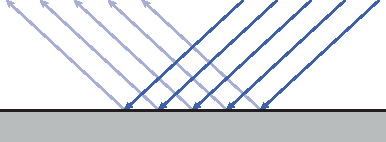
\includegraphics[width=.5\textwidth]{img/roughness0}
	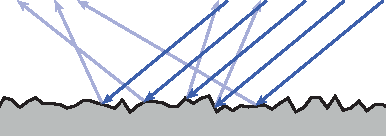
\includegraphics[width=.5\textwidth]{img/roughness1}
	\caption[Rauheit]{links: $m = 0$; rechts $m = 1$}
\end{figure}

Eines von ihnen ist das Cook-Torrance Modell \parencite{Cook1981}, welches mit dem Ziel entwickelt wurde die physikalischen Reflexionseigenschaften von rauhen und glatten Oberflächen realistischer abzubilden als es die klassischen Modelle ermöglichen \parencite[Seite 40]{Ngan2004}. Da sich das Cook-Torrance Modell auf spekulare Reflexionen konzentriert, verwenden wir das Cook-Torrance Modell auschließlich zur Berechnung des spekularen Anteils $f_s$ der BRDF. Der diffuse Anteil $f_d$ wird durch das klassische Lambert'sche Modell abgebildet und nicht weiter betrachtet. Denkbar sind aber auch andere Modelle für die diffuse Reflexion. In \fref{eq:cook-torrance-model} wird das Modell formal dargestellt.

\begin{align}
	\label{eq:cook-torrance-model}
	% \caption{Cook-Torrance Illumination}
	f_s(\mathbf V,\mathbf L) = \frac{\mathcal{F}(\mathbf V,\mathbf L)D(\mathbf V,\mathbf L)G(\mathbf V,\mathbf L)}{4(\mathbf N \cdot \mathbf V)(\mathbf N \cdot \mathbf L)}
\end{align}

Der spekulare Beitrag $f_s$ wird durch die drei Faktoren bestimmt: Dem Fresnel $\mathcal{F}$ Term, der Microfacet Richtungsverteilung, $\mathbf D$ und der geometrischen Abschwächung (Geometrical Attenuation) $\mathbf G$. Die Auswahl der konkreten Approximationen folgt der aus \cite[Seite 3]{Karis2013}.

\subsubsection[Fresnel]{Fresnel $\mathcal{F}$}
Der Fresnel Effekt beschreibt die Beobachtung, dass Oberflächen stärker reflektieren, umso flacher der Betrachtungswinkel wird. Als Approximation wurde die \textit{Schlick Approximation} \parencite{Schlick1994} gewählt. In \cite{Lagarde2012} wurde eine weitere Modifikation vorgeschlagen um den Berechnungsaufwand zu reduzieren. Diese findet hier ebenso ihre Anwendung.

\begin{align}
	\label{eq:fresnel-schlick}
	\mathcal F(\mathbf V,\mathbf L) = F_0  + (1 - F_0) 2^{(-5.55473 (\mathbf V \cdot \mathbf H) - 6.98316 (\mathbf V \cdot \mathbf H))}
\end{align}


\subsubsection[Facetten Normalverteilung]{Facetten Normalverteilung $D$} 
$D$ beschreibt die statistische Normalverteilung der Ausrichtung der Microfacets entsprechend der \warn{Winkelhalbierenden?} $H$. Die Microfacets von glatten Oberflächen sind überwiegend gleich ausgerichtet, so dass Licht hauptsächlich entlang $R$ reflektiert wird. Raue Oberflächen besitzen eher zufällig ausgerichtete Mircofacets, so dass das reflektierte Licht breiter gestreut wird. Die Rauheit der Oberfläche wird mit $m$ im Intervall $[0,1]$ ausgedrückt. Zur Approximation von $D$ finden sich wiederum eine vielzahl von Modelle. Die Implementierung verwendet das als \textit{GGX} in \cite{Walter2007} vorgestellte Modell (siehe \fref{eq:ggx}). $F_0$ beschreibt die Reflektanz für parallel zur Normale $\mathbf N$ einfallendes Licht.

\begin{align}
	\label{eq:ggx}
	D(\mathbf V,\mathbf L) = \frac{m^4}{ \pi \left(\left( \mathbf N \cdot \mathbf H \right)^2\left(m^4 - 1\right) + 1\right)^2}
\end{align}


\subsubsection[Geometrische Abschwächung]{Geometrische Abschwächung $G$} 
$G$ beschreibt einen Faktor, der die Tatsache simuliert dass Microfacets sich gegenseitig einfallendes oder reflektiertes Licht blockieren und sich somit gegenseitig schattieren ($G_1(\mathbf L)$) oder Reflexionen maskieren ($G_1(\mathbf V)$) können. Verwendet wird eine modifizierte Version der \textit{Schlick} Approximation, damit sie sich dem physikalisch präziseren Smith Modell annähert. Eine genauere Analyse des Smith Modells findet sich in \cite[Kapitel 6, Seite 33]{Heitz2014}.

\begin{align}
	\label{eq:geometric-schlick}
	k &= \frac{(m + 1)^2}{8}\\
	G_1(\mathbf V) &= \frac{\mathbf N \cdot \mathbf V}{(\mathbf N \cdot \mathbf V)(1-k)+k}\\
	G_1(\mathbf L) &= \frac{\mathbf N \cdot \mathbf L}{(\mathbf N \cdot \mathbf L)(1-k)+k}\\
	G(\mathbf V,\mathbf L) &= G_1(\mathbf V) G_1(\mathbf L)
\end{align}


\subsubsection{Dielektische und metallische Materialien}

In der Natur lassen sich Substanzen bezüglich ihrer Leiteigenschaften in drei Kategorien einteilen: Nichtleiter (Dielektrikum oder Isolatoren), Halbleiter und Leiter (u.A. metallische Substanzen). Ohne auf die physikalischen Details einzugehen (\warn{Ref}) unterscheiden sich metallische und dielektrische Materialien in ihrem spekularem Reflexionsverhalten. Dielektrische Materialien besitzen ausschließlich weiße spekulare Reflexionen (siehe \warn{bild}) während metallische Materialien über ein Farbspektrum spekular reflektieren \parencite[Abschnitt: Specular]{Lagarde2011a}.

In der Implementierung bilden wir das über eine Justierung des $F_0$ Wertes aus dem Fresnel-Term $\mathcal{F}$ ab. Für metallische Materialien setzen wir $F_0$ auf die Grundfarbe des Materials, ansonsten setzen wir wie $F_0$ auf weiß (Idee basiert auf der Unreal Engine 4 Implementierung, Stand 2014).

\section{Praktische Umsetzung}
\label{sec:pbr-umsetzung}

Wie Eingangs erwähnt erfordert die Umstellung auf \ac{PBR} eine Anpassung der Produktions- und Renderpipeline. Während Diffuse- bzw Albeo-Texturen sowie Normalentexturen bereits üblich sind, ist es für die Albedo Texturen um so wichtiger, dass die von jeglicher \"eingebackener\" Beleuchtung bereinigt sind (Details in \cite{Lagarde2011}), damit die grundlegenden Texturen in allen Beleuchtungssituationen funktionieren. Die Implementierung wird im \fref{chap:anwendung} auszugsweise vorgestellt. Im Folgenden eine kurze Übersicht über die praktischen Grundlagen der Implementierung.

\subsection{Eingangsparameter}

Als Eingangsparameter verwendet die Pipeline der Implementierung dieser Arbeit folgende Größen:
\begin{itemize}
\item Albedo-Textur im sRGB Farbraum
\item Normalen-Textur mit Oberflächennormale im Tangent-Raum kodiert in RGB
\item Roughness-Textur ($m$) in Graustufen
\item Metallic-Textur in Graustufen für die Unterscheidung von dielektrischen und metallischen Oberflächen\footnote{Entspricht einer Maske, 0 = nicht metallisch, 1 = metallisch}
\end{itemize}

\subsection{Renderverfahren}

Als Renderverfahren wurde das als \textit{Deferred Shading} bekannte Verfahren gewählt, da es effizienter als \textit{Forward Shading} in der Lichtberechnung von vielen Lichtern ist. Dazu wird vor der Berechnung der Schattierung der Oberflächen die Geometrie gerendert. In diesem Renderschritt werden die Oberflächenattribute wie Albedo-Farbe, Roughness und Normale in Texturen gerendert, kombiniert oft \textit{G-Buffer} genannt. Dieser \textit{G-Buffer} dient dann anschließend im Shading Renderschritt als Grundlage für die Berechnung. In diesem Schritt werden die Lichter mit Stellvertreter Geometrien gerendert. Für jedes so erzeugte Fragment wird dann die gewählte \ac{BRDF} mit Hilfe der Lichtparameter und der Parameter aus dem G-Buffer ausgewertet. In der fortlaufenden Pipeline werden die Farbwerte im HDR-Raum behandelt. Im abschließenden sogenannten Tone-Mapping Schritt werden die Farbwerte vom HDR-Raum auf den linearen (s)RGB Raum übertragen. Weiterführende Details finden dazu finden sich in der Implementierung zu dieser Arbeit oder in \cite{Shishkovtsov2005}.

\subsection[Indirekte Beleuchtung]{Indirekte Beleuchtung mit \acl{IBL}}

Bisher wurde nur die direkte Beleuchtung von Materialien betrachtet. Aber ein weiterer wesentlicher Beitrag zum realistischen Eindruck ist die sogenannte indirekte Beleuchtung. Indirekte Beleuchtung beschreibt physikalische Tatsache, dass Objekte nicht nur direkt von Lichtquellen beleuchtet werden, sondern selbst wieder Licht reflektieren. Entweder trifft das reflektierte Licht in das Auge des Betrachters, so dass Objekte für uns sichtbar werden, oder wiederum auf andere Objekte. Letzteres führt dazu, dass Oberflächen durch das von anderen Oberflächen reflektierte Licht zusätzlich beleuchtet werden \warn{Bild}. Diese wechselseitige Interreflexion wird unter dem Begriff indirekte Beleuchtung zusammengefasst.

Bisher haben wir in \fref{eq:brdf-dekonstruiert} ausschließlich die \ac{BRDF} mit direkter Beleuchtung betrachtet, aber die \ac{BRDF} lässt sich wie in \fref{eq:brdf-indirect-dekonstruiert} um Beiträge aus ambienten bzw. indirekten Beleuchtungstermen erweitern. Da spekulare Reflexionen kein Sonderfall sind \parencite{Hable2010}, lohnt es sich ein generelles Verfahren zur Berechnung des indirekten Beitrags $f_{indirect}$ zu wählen. 

\begin{align}
	% \caption{Dekonstruierte BRDF}
	\label{eq:brdf-indirect}
	f   &= f_d + f_s\\
	\intertext{Erweiterung von $f_d$ und $f_s$ um ambienten Beitrag:}
	{f_d}^{\prime} &= f_{d_{indirect}} + f_{d_{direct}}\\
	{f_s}^{\prime} &= f_{s_{indirect}} + f_{s_{direct}}\\
	\label{eq:brdf-indirect-dekonstruiert}
	f^{\prime}   &= \underbrace{f_{d_{indirect}} + f_{s_{indirect}}}_{f_{indirect}} + \underbrace{f_{d_{direct}} + f_{s_{direct}}}_{f_{direct}}
\end{align}

Idealerweise lässt sich die Pipeline um ein umfassendes \acf{GI}\footnote{\acl{GI} Synonym für indirekte Beleuchtung.} Verfahren erweiteren, dass die wechselseitigen Interreflexionen aller Objekte im Raum über ein möglichst breites Frequenzenband\footnote{niedrige Frequenzen = diffuse Reflexion $f_{d_{indirect}}$; hohe Frequenzen = spekulare Reflexion $f_{s_{indirect}}$} hin abdeckt. Doch voll dynamisches \ac{GI} ist immer noch in Echtzeit nicht vollends praktikabl, und ist aktuell nur auf Highend Hardware, wie zum Beispiel über Verfahren wie \ac{SVOGI} \parencite{Lin2013}, zu realisieren.

Entsprechend suchen wir nach einer vereinfachten Möglichkeit, generelle Reflexionen in unterschiedlichen Frequenzen abzubilden. Zum Einsatz kommt hier ein erweitertes \acf{IBL} Verfahren, dass die Umgebungstexturen im Preprozess für die unterschiedlichen Frequenzen vorintegriert. Die Vorintegration läuft aktuell noch nicht direkt in der Pipeline ab sondern wird offline mit dem von Sébastien Lagarde modifiziertem Programm \textit{AMD Cubemapgen} durchgeführt \parencite{Lagarde2012a}. Dazu wird eine HDR-Cubemap in das Programm geladen und mit den passenden Einstellungen gefiltert. Das Resultat ist eine \ac{PMREM} die dann geladen und in der Auswertung der \ac{BRDF} verwendet wird.\warn{PMREM erläutern}.

\section{Wo wird es eingesetzt?}
\label{sec:pbr-wo}
Inzwischen wird das Verfahren in allen großen Spieleengines eingesetzt: CryEngine \parencite{Schulz2014}, Unreal Engine 4 \parencite{Martin2012}, Frostbite \parencite{Lagarde2014}, der Engine hinter den Call of Duty Titeln \parencite{Lazarov2011} und EVE Online \parencite{CCP2014}.
